% ============================================================
% LLM-BLM 補足実験 X02〜X04：共分散の窓、TE の上限の校正、VIX
% コンパイル：tectonic -X compile LLM-BLM_補足実験_共分散とTE.tex   （XeTeX 系。このフォルダで実行する）
% 図は 図/（作成スクリプト/figs.py が experiments/X02〜X04 の results から作る）
% 数値の出どころは各実験の results/summary.json と findings.md
% ============================================================
\documentclass[xelatex,ja=standard,jafont=haranoaji,a4paper,10pt,openany]{bxjsreport}
\setpagelayout*{left=24mm,right=24mm,top=24mm,bottom=26mm,footskip=11mm}

\usepackage{amsmath,amssymb,mathtools,bm}
\usepackage{booktabs,array,multirow,longtable}
\usepackage{graphicx}
\usepackage{adjustbox}
\usepackage{xcolor}
\usepackage{tikz}
\usetikzlibrary{arrows.meta,positioning,calc,fit}
\usepackage{enumitem}
\usepackage{caption}
\usepackage{float}
\usepackage[most]{tcolorbox}
\usepackage[hidelinks,bookmarksnumbered]{hyperref}
\pdfstringdefDisableCommands{\def\Omega{Ω}\def\tau{τ}\def\Sigma{Σ}}

\graphicspath{{図/}}

\definecolor{c1}{HTML}{2A78D6}
\definecolor{c2}{HTML}{EB6834}
\definecolor{c3}{HTML}{1BAF7A}
\definecolor{c4}{HTML}{EDA100}
\definecolor{c7}{HTML}{6250D6}
\definecolor{ink2}{HTML}{52514E}
\definecolor{soft1}{HTML}{E4EEF9}
\definecolor{soft2}{HTML}{FBEEDF}
\definecolor{soft3}{HTML}{E3F3E9}
\definecolor{soft4}{HTML}{EEE8FA}
\definecolor{soft5}{HTML}{FDF3DA}

\newcommand{\code}[1]{\texttt{#1}}
\newcommand{\SP}{S\&P500}
\newcommand{\figref}[1]{図~\ref{#1}}
\newcommand{\tabref}[1]{表~\ref{#1}}
\newcommand{\chapref}[1]{第~\ref{#1}~章}
\newcommand{\secref}[1]{\ref{#1}~節}

\setlist[itemize]{leftmargin=1.6em,itemsep=0.2em,topsep=0.4em}
\setlist[enumerate]{leftmargin=1.8em,itemsep=0.2em,topsep=0.4em}
\captionsetup{font=small,labelfont=bf,skip=6pt}
\renewcommand{\arraystretch}{1.2}
\setlength{\LTpre}{6pt}
\setlength{\LTpost}{6pt}

\makeatletter
\def\@makechapterhead#1{\vspace*{0.3\Cvs}{\parindent\z@\raggedright\normalfont
  \ifnum\c@secnumdepth>\m@ne\if@mainmatter{\Large\headfont\@chapapp\thechapter\@chappos}\par\nobreak\vskip0.4\Cvs\fi\fi
  \interlinepenalty\@M\LARGE\headfont #1\par\nobreak\vskip 1.5\Cvs}}
\def\@makeschapterhead#1{\vspace*{0.3\Cvs}{\parindent\z@\raggedright\normalfont
  \interlinepenalty\@M\LARGE\headfont #1\par\nobreak\vskip 1.5\Cvs}}
\makeatother

\newtcolorbox{keybox}[1][要点]{enhanced,breakable,colback=soft1,colframe=c1,boxrule=0.5pt,arc=2pt,
  left=8pt,right=8pt,top=6pt,bottom=6pt,title={#1},fonttitle=\sffamily\bfseries\small,coltitle=white}
\newtcolorbox{notebox}[1][注意]{enhanced,breakable,colback=soft2,colframe=c2,boxrule=0.5pt,arc=2pt,
  left=8pt,right=8pt,top=6pt,bottom=6pt,title={#1},fonttitle=\sffamily\bfseries\small,coltitle=white}
\newtcolorbox{verdict}[1][判定]{enhanced,breakable,colback=soft4,colframe=c7,boxrule=0.5pt,arc=2pt,
  left=8pt,right=8pt,top=6pt,bottom=6pt,title={#1},fonttitle=\sffamily\bfseries\small,coltitle=white}

\tikzset{
  box/.style={draw=#1,fill=#1!8,rounded corners=2pt,align=center,font=\footnotesize,inner sep=4pt,
              minimum height=10mm,text width=24mm},
  arr/.style={-{Stealth[length=2mm]},color=ink2,line width=0.6pt},
}

\title{LLM-BLM 補足実験 X02〜X04\\[6pt]
  \large BLM の TE の約束を守るには：\\共分散の窓、上限の校正、VIX}
\author{実験の結果の報告書}
\date{2026 年 10 月 18 日}

\begin{document}
\maketitle

% ============================================================
\chapter*{概要}
\addcontentsline{toc}{chapter}{概要}

BLM の最適化では、事前の TE（トラッキングエラー、時価総額の比率からのずれの大きさ）を年 3\% 以下に抑えている。ところが X01（実験 2 の報告書の付録）で、実際の TE は約 4.5\% と、約束の約 1.5 倍になっていた。この報告書では、そのずれを直す方法を 3 つの実験で比べた。LLM は使わず、仮の見通し（12-1 か月のモメンタム）で BLM を動かした。どの実験も、比べ方をスクリプトに書いてコミットしてから 1 回だけ実行した。

\begin{keybox}[主な結論]
\begin{itemize}
\item \textbf{X02 共分散の窓を変えても、ずれはほとんど直らない。}一番良い指数の重み（半減期 126 日）でも、実際の TE は 4.26\%（約束の 1.42 倍）。今の 252 日（4.58\%）より少し良いだけだった。
\item \textbf{X03 上限を過去の「実際 ÷ 予測」の比で割ると、約束が守れる。}上限は約 2\% になり、実際の TE は 4.79\% から 3.38\%（中央値 3.20\%）に下がった。3\% からのずれは半分以下になった（$t=-6.5$）。将来のデータは使わない。
\item \textbf{X04 VIX で共分散の大きさを合わせても、上の校正より良くならない。}2020 年 2 月の暴落の月には効いた（7.5\% → 5.2\%）が、全体では有意な改善はなかった。
\end{itemize}
\end{keybox}

\textbf{BLM への反映}：共分散は Ledoit--Wolf のまま、TE の上限に X03 の校正を入れる。実験 7（月次の BLM）では、この校正で実際の TE が 2.5\% と約束の内に収まった。

\setcounter{tocdepth}{1}
{\small\tableofcontents}

% ============================================================
\chapter{問題：TE の約束が守られていない}\label{ch:intro}

BLM は、見通しに合わせて時価総額の比率から少しずらした比率を作る。ずらし過ぎないように、事前の TE（共分散 $\Sigma$ から計算した、時価総額とのリターンの差の標準偏差）を年 3\% 以下に抑える。

X01 で、2016〜2026 年の 127 か月について、翌月の実際の TE を測った。どの共分散の推定でも、実際は 4.5〜4.8\% だった。原因として考えられるのは次の 2 つである。

\begin{enumerate}
\item \textbf{リスクの変化を捉えられない。}共分散は過去 1 年から推定するので、翌月にリスクが急に変わると（2020 年 3 月など）外れる。
\item \textbf{最適化が推定の誤差を利用する。}最適化は、リスクが小さく見える組み合わせを選ぶ。その組み合わせは、推定の誤差で小さく見えているだけのことが多い（最適化の呪い）。
\end{enumerate}

\section{共通の設定}

\begin{itemize}
\item \textbf{銘柄}：各月末の \SP{} の構成銘柄（平均 463 銘柄）。
\item \textbf{期間}：判断日は月末。X02 は 2017-01〜2026-07 の 115 か月、X03・X04 は 2020-01〜2026-07 の 79 か月（過去 36 か月の比が計算できる月から）。
\item \textbf{BLM の最適化}：均衡リターン ＋ 仮の見通し（IC 0.05 × ボラティリティ × モメンタムの正規スコア）、リスク回避度 2.5、事前の TE の上限つき、空売りなし。
\item \textbf{共分散}：Ledoit--Wolf の縮小推定（今の BLM と同じ）。
\end{itemize}

% ============================================================
\chapter{X02：共分散の窓}\label{ch:x02}

\section{比べたもの}

直近 63・126・252（今）・504 取引日を同じ重みで使う 4 通りと、直近 504 日を指数の重み（半減期 63 日・126 日）で使う 2 通りの、計 6 通り。どれも Ledoit--Wolf で縮小した。

\section{結果}

\begin{figure}[H]
\centering
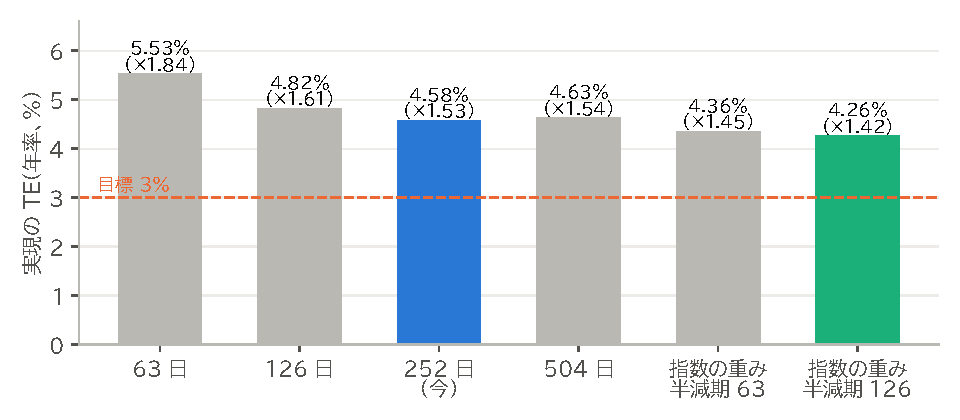
\includegraphics[width=0.86\linewidth]{x02_te.pdf}
\caption{各推定で BLM を作ったときの、翌月の実際の TE の平均（115 か月）。括弧は「実際 ÷ 約束」。}
\label{fig:x02}
\end{figure}

\begin{itemize}
\item 指数の重み（半減期 126 日）が一番良く、実際の TE は 4.26\%。今の 252 日より 0.32 ポイント低く（$t=-11.5$）、85\% の月で良かった。
\item それでも約束の 1.42 倍で、窓ではずれの大部分が残る（\figref{fig:x02}）。
\item 短い窓（63 日）は大きく悪い（5.53\%）。推定のノイズが増え、最適化がそれを利用する。
\end{itemize}

\begin{notebox}[設計の誤り]
事前に決めたもう 1 つの指標（252 日で作った比率のリスクの当たり具合、QLIKE）は、252 日に不利な比べ方だった。その比率は 252 日で最適化したので、252 日が一番リスクを小さく見積もる向きに寄っている。実行の前に気づけなかった。どの推定にも同じ比率（時価総額・等金額）で比べ直すと、推定の間に有意な差はなかった（$|t|<1.9$）。
\end{notebox}

% ============================================================
\chapter{X03：上限の校正}\label{ch:x03}

\section{規則}

各判断日に、直近 36 か月（どれも保有が終わっている）の「実際の TE ÷ 事前の TE」の平均で、3\% を割った値を事前の上限にする。将来のデータは使わない。比はおおむね 1.4〜1.6 で安定していて、上限は平均 1.93\%（252 日）と 2.07\%（指数の重み 126 日）になった。

\section{結果}

\begin{figure}[H]
\centering
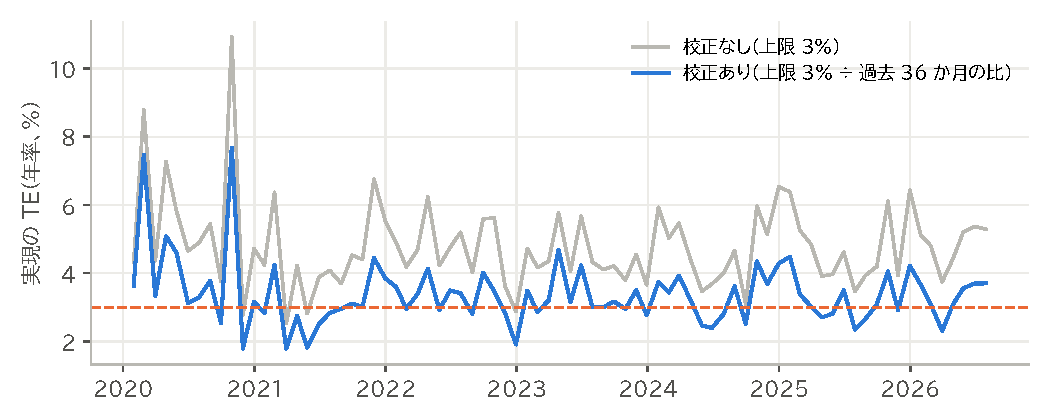
\includegraphics[width=0.92\linewidth]{x03_series.pdf}
\caption{252 日の推定での、月ごとの実際の TE。灰色は校正なし、青は校正あり。破線は約束の 3\%。}
\label{fig:x03}
\end{figure}

\begin{table}[H]
\centering
\caption{校正の効果（同じ 79 か月）。}
\small
\begin{tabular}{lrrrr}
\toprule
& \multicolumn{2}{c}{252 日（今）} & \multicolumn{2}{c}{指数の重み 126 日} \\
& 校正なし & 校正あり & 校正なし & 校正あり \\
\midrule
実際の TE の平均 & 4.79\% & \textbf{3.38\%} & 4.44\% & \textbf{3.28\%} \\
同・中央値 & 4.55\% & 3.20\% & 4.16\% & 3.06\% \\
3\% からのずれ（RMSE） & 2.20 & \textbf{1.03} & 1.90 & \textbf{1.02} \\
ずれの 2 乗の差の $t$ & & $-6.5$ & & $-5.5$ \\
3\% を超えた月 & 95\% & 66\% & 94\% & 53\% \\
超過リターン（年率） & $+1.16\%$ & $+0.96\%$ & $+1.42\%$ & $+1.07\%$ \\
情報比 & 0.28 & 0.32 & 0.37 & 0.37 \\
\bottomrule
\end{tabular}
\end{table}

\begin{itemize}
\item 校正で 3\% からのずれが半分以下になった。
\item リスクを小さくした分、超過リターンは減るが、リスクあたり（情報比）は変わらないか、わずかに良くなった。
\item 平均がまだ 3\% を少し上回るのは、2020 年 2〜4 月と 10 月の大きく外れた月のため（\figref{fig:x03}）。
\end{itemize}

この校正は、市販のリスクモデル（MSCI Barra の USE4）の「最近の実際と予測の比で予測を引き上げる」調整と同じ発想である。

% ============================================================
\chapter{X04：VIX で共分散の大きさを合わせる}\label{ch:x04}

\section{やったこと}

X03 で残ったのは、ボラティリティが急に変わる月だった。VIX は、\SP{} のオプション価格から読み取った、翌 30 日のボラティリティの市場予想である。各判断日に共分散の全体を $k$ 倍し、時価総額の比率の予測ボラティリティを、その日の VIX に一致させた（$k$ は 0.4〜9.3 倍、2020-02-28 は約 9 倍）。VIX だけの場合と、X03 の校正と組み合わせた場合を比べた。

\section{結果}

\begin{figure}[H]
\centering
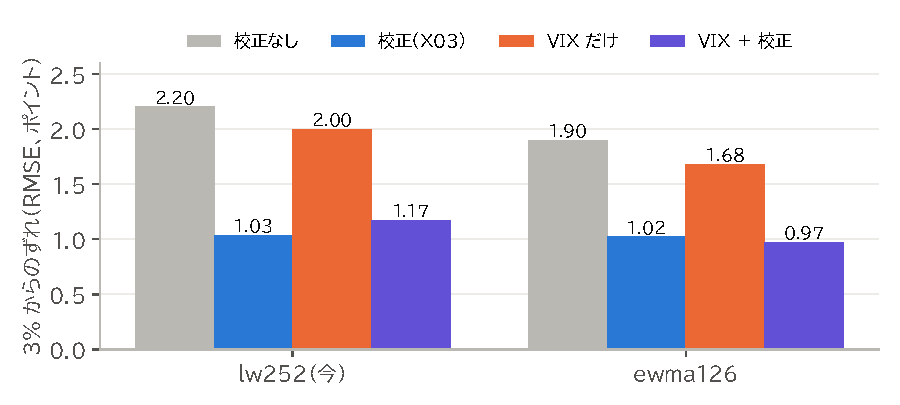
\includegraphics[width=0.8\linewidth]{x04_rmse.pdf}
\caption{3\% からのずれ（RMSE、ポイント。2020-01〜2026-07 の 79 か月）。}
\label{fig:x04}
\end{figure}

\begin{figure}[H]
\centering
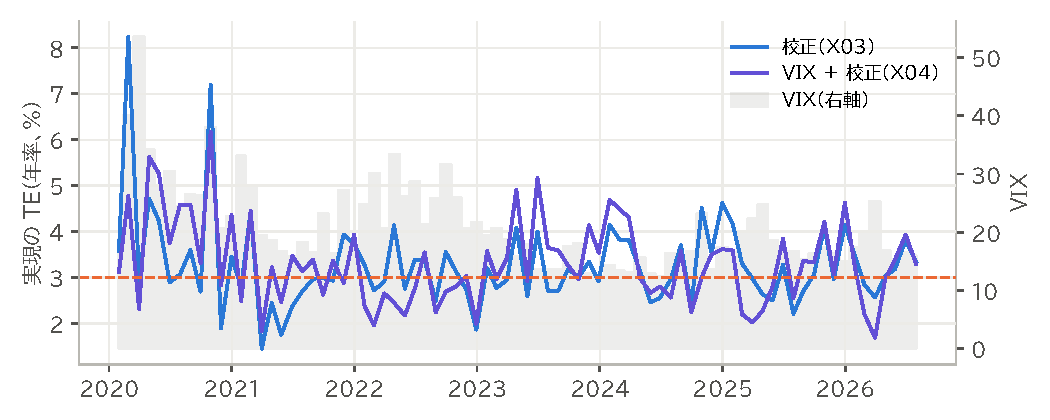
\includegraphics[width=0.92\linewidth]{x04_series.pdf}
\caption{指数の重み 126 日での、月ごとの実際の TE。青は X03 の校正、紫は VIX ＋ 校正。灰色は VIX（右軸）。}
\label{fig:x04s}
\end{figure}

\begin{verdict}
\textbf{支持されない。}校正に VIX を加えても、ずれは有意に減らない（252 日で $t=1.1$、指数の重みで $t=-0.3$）。良くなった月は 38〜41\% だけだった（\figref{fig:x04}）。
\end{verdict}

\begin{itemize}
\item \textbf{暴落の月には効いた。}2020 年 2 月は、252 日で 7.5\% → 5.2\%、指数の重みで 8.2\% → 4.8\%。VIX が先に跳ねたので、最適化がずれを抑えた。
\item \textbf{それ以外の外れには効かない。}2020 年 10 月は、市場全体は落ち着いていたが、業種の間の入れ替わりが激しかった（\figref{fig:x04s}）。
\item \textbf{理由}：VIX は市場全体のぶれを予想する。TE は時価総額とのずれ、つまり銘柄の間のばらつきなので、VIX だけでは捉えきれない。落ち着いた月には VIX が低く、上限が実質的に緩んで少し悪くなる。
\end{itemize}

% ============================================================
\chapter{まとめと限界}\label{ch:summary}

\section{BLM への反映}

\begin{enumerate}
\item 共分散は Ledoit--Wolf のまま（指数の重み 126 日にすると少し良いが、差は小さい）。
\item TE の上限は、過去 36 か月の「実際 ÷ 予測」の比で 3\% を割る（X03）。
\item VIX での調整は入れない。暴落の月だけ効くが、その規則を結果を見てから作ると過剰適合になる。
\end{enumerate}

実験 7（LLM の見通しの月次の BLM）では、この校正で上限が平均 1.95\% になり、実際の TE は 2.46\% と約束の内に収まった。

\section{限界}

\begin{itemize}
\item 期間は 1 つ（X03・X04 は 2020〜2026 年）。大きく外れる月は数か月しかない。
\item 見通しは仮のモメンタム。LLM の見通しでは比が違いうる（実験 7 では校正が働いた）。
\item 校正の規則は 1 つ（36 か月の平均）だけ試した。期間などを選び直すと過剰適合になる。
\end{itemize}

% ============================================================
\chapter*{再現の手順}
\addcontentsline{toc}{chapter}{再現の手順}

\begin{verbatim}
python experiments/X02_covariance_window/run.py   # コミット f48f358 で固定
python experiments/X03_te_calibration/run.py      # コミット 29711dc で固定
python experiments/X04_vix_scaling/run.py         # コミット d8529f9 で固定
cd 資料集/02_実験/補足実験_共分散とTE
python 作成スクリプト/figs.py                      # この資料の図
\end{verbatim}

数値の出どころは、各実験の \code{results/summary.json}、月ごとの CSV、\code{findings.md}。費用は 0 円（CPU で数分ずつ）。

\end{document}
